%----------------------------------------------------------------
%
%  File    :  vpn_fuzzing.tex
%
%  Author  :  Benjamin Wunderling, TU Graz, Austria
% 
%  Created :  22 Feb 96
% 
%  Changed :  19 Feb 2004
% 
%----------------------------------------------------------------

\chapter{Fuzzing}

\label{chap:Fuzzing}

\iffalse
\section{Environment Setup} \label{sec:fuzzenv}
% describe VMs, IPsec server software, configuration etc
We ran all our fuzzing tests in the same virtual network setup we used for our automata learning, on the same Ubuntu 22.04 LTS distributions. We again designated one \ac{vm} as the initiator which would send the fuzzed messages and the other one as the responder to create a typical client-server setup. All settings on the used VMs remained the same as while learning to ensure that no discrepancies were introduced by different environment settings. The \ac{sut} was also the same Strongswan server used for learning. The major difference to learning is that for fuzzing, we no longer require \textsc{AALpy}. Our only real dependency, apart from our mapper class, is the Python fuzzing framework boofuzz, version 0.4.1, which we use for input generation. 
\fi

This chapter presents our model-based fuzzing setup used to test a Strongswan \ac{ipsec} server. It first gives a high-level overview of our fuzzing process and then goes into more detail on the individual involved components and methodologies. We focus on testing entire input sequences (sequences of inputs of the input alphabet), and present two different methods of generating input sequences for fuzzing, with an emphasis on reducing the total runtime of fuzzing to a reasonable amount.

\section{Fuzzing Setup} \label{sec:fuzz_intro}
A basic fuzzing loop consists of test data generation, execution on the \ac{sut} and observing the \ac{sut} for strange behavior. Applied to fuzzing an \ac{ipsec} server in a potential black-box scenario, some additional considerations and steps are required, as seen in Figure~\ref{fig:fuzz_overview}. Firstly, it must be taken into consideration, that the \ac{sut} reacts differently to inputs depending on which state it is in and a lot of states are locked behind specific sequences of valid inputs (e.g. phase two requiring a prior successful phase one). Therefore, it stands to reason that in order to achieve good coverage of \ac{sut} functionality, the \ac{sut} must be put into specific states prior to receiving each fuzzed test case. To this end, specific input sequences are passed to the fuzzer, which, at random, chooses a single input of each input sequence to fuzz, while still sending the other unchanged inputs surrounding the fuzzed input to the \ac{sut} as well.
Note that technically, the mapped concrete \ac{isakmp} packet is fuzzed and not the abstract input, as is explained in more detail in Subsection~\ref{subsec:sequence_generation}, however, we will continue to refer to it as the ``fuzzed input''.
Additionally, the \ac{sut} is reset after each execution of a fuzzed input sequence, ensuring that each fuzzed input is executed in exactly the same starting state of the \ac{sut}. Figure~\ref{fig:fuzz_overview} shows an example of such a fuzzed input sequence, with the fuzzed input being the third input of the sequence. In order to be able to detect strange behavior, a Mealy machine implementation of a learned reference model of the \ac{sut} is created, depicted in yellow in Figure~\ref{fig:fuzz_overview}. Each input that is sent to the \ac{sut}, depicted in red in Figure~\ref{fig:fuzz_overview}, is also executed on the Mealy machine in parallel, comparing the response codes of the \ac{sut} and Mealy machine. A mismatch between the response of the \ac{sut} and the expected one returned by the Mealy machine indicates, that a new state or behavior has been discovered. As the Mealy machine was created from the model of the \ac{sut}, any new behavior can be treated as interesting behavior worth further investigation. Input sequence generation/selection, new state detection and fuzz input generation is all handled separately from the \ac{sul} interface, in a new script called \emph{fuzzing.py}~\footnote{TODO: github or supplementary material link}.

\begin{figure}
\begin{centering}
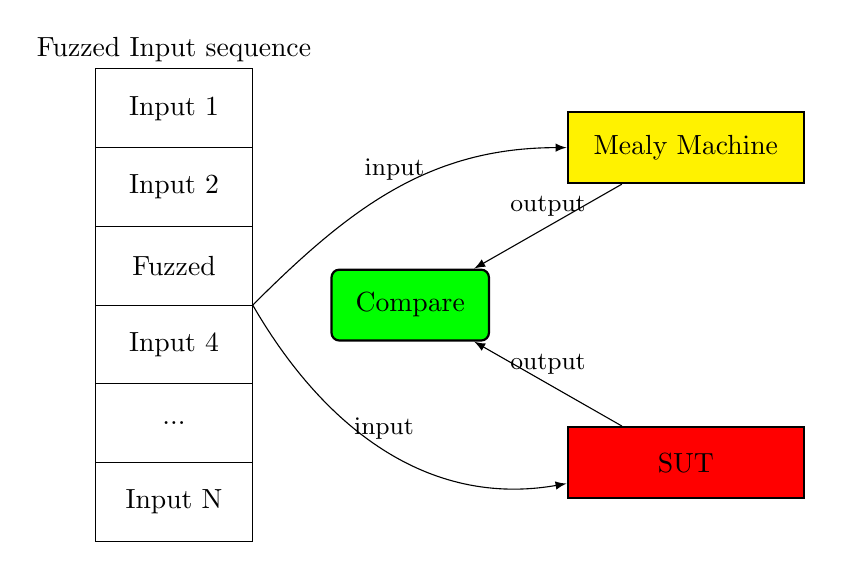
\begin{tikzpicture}
		\node (title) at (1,6.25) {Fuzzed Input sequence};
		\node (0) at (0, 6) {};
		\node (1) at (0, 5) {};
		\node (2) at (0, 4) {};
		\node (3) at (0, 3) {};
		\node (4) at (0, 2) {};
		\node (5) at (0, 1) {};
		\node (6) at (0, 0) {};
		\node (7) at (2, 0) {};
		\node (8) at (2, 1) {};
		\node (9) at (2, 2) {};
		\node (10) at (2, 3) {};
		\node (11) at (2, 4) {};
		\node (12) at (2, 5) {};
		\node (13) at (2, 6) {};

		\node (sut) at (7.5, 1) [draw,thick,minimum width=3cm,minimum height=0.9cm, fill=red] {SUT};
		\node (26) at (1, 2.5) {Input 4};
		\node (27) at (1, 5.5) {Input 1};
		\node (28) at (1, 4.5) {Input 2};
		\node (29) at (1, 3.5) {Fuzzed};
		\node (30) at (1, 1.5) {...};
		\node (31) at (1, 0.5) {Input N};
		\node (32) at (6, 6) {};
		\node (33) at (6, 4) {};
		\node (34) at (9, 4) {};
		\node (35) at (9, 6)  {};
		\node (sm) at (7.5, 5) [draw,thick,minimum width=3cm,minimum height=0.9cm, fill=yellow] {Mealy Machine};
		\node (37) at (2, 3) {};
		\node (39) at (6, 0.5) {};
		\node (40) at (6, 4.75) {};
		\node (comp) at (4, 3) [draw,thick,minimum width=2cm,minimum height=0.9cm,rounded corners=.1cm, fill=green] {Compare};
		\node (42) at (6, 1.5) {};

		\draw [in=180, out=0] (0.center) to (13.center);
		\draw (0.center) to (1.center);
		\draw (1.center) to (2.center);
		\draw (2.center) to (3.center);
		\draw (3.center) to (4.center);
		\draw (4.center) to (5.center);
		\draw (5.center) to (6.center);
		\draw (6.center) to (7.center);
		\draw (7.center) to (8.center);
		\draw (8.center) to (9.center);
		\draw (9.center) to (10.center);
		\draw (10.center) to (11.center);
		\draw (11.center) to (12.center);
		\draw (12.center) to (13.center);
		\draw (1.center) to (12.center);
		\draw (2.center) to (11.center);
		\draw (3.center) to (10.center);
		\draw (4.center) to (9.center);
		\draw (5.center) to (8.center);
		\draw[-latex] (37.center) to [out=45,in=180] node[pos=0.5, above, font=\small]{input} (sm);
		\draw[-latex](37.center) to [out=300,in=190] node[pos=0.5, above, font=\small]{input} (sut);
		\draw[-latex] (sm) -- node[pos=0.5, above, font=\small]{output} (comp);
		\draw[-latex] (sut) -- node[pos=0.5, above, font=\small]{output} (comp);
		
\end{tikzpicture}
\caption{Overview of the fuzzing process.}
\label{fig:fuzz_overview}
\end{centering}
\end{figure}

While this basic fuzzing procedure is rather straightforward, the questions remaining is how to choose or generate the input sequences that are to be fuzzed, how the reference model is created/learned and how the test data for fuzzed inputs in generated. The following subsections cover the creation of the reference model, as well as two methods of input sequence selection/generation.

\subsection{Learning the Reference Model} \label{subsec:adapting_model}
The black-box determination of interesting inputs during fuzzing requires a model of the \ac{sut} to extract expected responses from. While a (deterministic) model of the \ac{sul} when exposed to expected inputs, had already successfully been learned, this proved to be not particularly useful for model-based fuzzing, as the majority of fuzzed inputs would result in an error message response from the \ac{sut} and therefore be treated as a new state. Instead of using the model of only expected behavior, a new model was learned, again using retransmission-filtering, but this time also with an expanded input alphabet. In addition to the previous input alphabet, an erroneous version of each input was added, that maps to an \ac{ike} packet with some sort of error or malformation. An example of such a malformed packet could be an incorrect length field, a wrong hash value or simply an unsupported \ac{sa} option. Adding these new inputs to our input alphabet doubles its size and results in the following input alphabet: \emph{sa\_main}, \emph{key\_ex\_main}, \emph{authenticate}, \emph{sa\_quick}, \emph{ack\_quick}, \emph{sa\_main\_err}, \emph{key\_ex\_main\_err}, \emph{authenticate\_err}, \emph{sa\_quick\_err} and \emph{ack\_quick\_err}. The model learned using the new input alphabet represents the behavior of the \ac{sul} when exposed to expected inputs, as well as unexpected inputs, that could arise during fuzzing. Since our mapper class was designed in such a way as to allow for easy manipulation of packets, this was an easy change to implement. Some additional server responses had to be parsed correctly, but all in all, not much had to be changed in our mapper class to allow for the sending of erroneous packets. 


\subsection{Detecting New States} \label{subsec:state_detect}
As inputs should be executable simultaneously on the \ac{sut} as well as on the reference model and have their respective responses compared in order to discover new states, i.e. new behavior. In order to be able to compare the outputs automatically, a Python representation of the learned reference model is required. Conveniently, \textsc{AALpy} is able to parse generated dot files into a corresponding Mealy machine object. This Mealy machine has a current state, as well as a \texttt{step} method, taking an abstract input as a parameter and returning the corresponding expected response based on the learned response when applying that input to the current state. Using this Mealy machine, a fuzzed input sent to the \ac{sut} can then easily be checked to see if it results in the same next state and response as it did on our reference model. By passing the same input to both the actual \ac{sut} and the Mealy machine representation of the reference model, this comparison becomes very simple and can be easily automated. If the two responses do not match, a new state and therefore hitherto unexplored behavior of the \ac{sut} will have been discovered. 

Using the Mealy machine representation of our new reference model, we were able to filter out the expected standard error correcting behavior and instead focus on more unusual behavior than previously. 

\subsection{Test Data Generation} \label{subsec:data_gen}
As our mapper class was designed to allow for the easy fuzzing of \ac{ipsec} fields, the only thing missing for test case generation is a source of values to use for fuzzing the individual fields. Our choice was the open source fuzzing library boofuzz\footnote{\url{https://github.com/jtpereyda/boofuzz}}, which is a successor of the popular Sulley\footnote{\url{https://github.com/OpenRCE/sulley}} fuzzing framework. Boofuzz is usually used by first defining a protocol in terms of blocks and primitives that define the contents of each message, and then using those definitions to generate large amounts mutated values for testing. However, as our mapper class already had a very flexible way of sending manipulated \ac{ipsec} packets and the protocol structure is quite rigid, we decided to only use the data generation features of boofuzz, which are mutation-based, forgoing the protocol definitions. To get relevant fuzz values for each field, every fuzzable field was mapped to a matching boofuzz primitive data type and then used that to generate our data. This ensures that each field is fuzzed with relevant data allowed by the protocol, e.g. string inputs are not suddenly used for length fields. While testing completely incompatible types of inputs would also be an interesting experiment in and of itself, we decided to focus on allowed but unexpected inputs, as these seemed the most likely to lead to undocumented/unexpected behavior. Additionally, supporting completely invalid types would have required a complete redesign of our mapper class. To summarize, we now have a rough fuzzing framework, consisting of a reference model to detect new states reached during fuzzing, as well as fuzz data generation, on a field type-by-field type basis. However, we are still missing a way of choosing which, or generating input sequences to insert the fuzzed test data into. 


\subsection{Input Sequence Generation} \label{subsec:sequence_generation}
% tools used
The final piece missing for our fuzzer is the input sequence-generation phase, in which a set of input sequences is generated/selected. During fuzzing, one (or more) of the inputs in the input sequence will be chosen to be fuzzed. An input is fuzzed, by replacing certain interesting fields of the concrete \ac{isakmp} packet it maps to, with fuzzed values. Fuzzed inputs are embedded in a full input sequence to ensure that the fuzzed input is always executed in the same state, provided the \ac{sut} is reset after each sent/received input sequence. The difficulty lies in selecting or generating the input sequences to use for fuzzing in such a way, that the amount of new states discoverable through fuzzing is maximized, i.e. as much interesting new behavior is tested as possible. Effectively, this means that the goal is to achieve good coverage of the interesting behavior of the \ac{sut}. As the \ac{sut} is a reactive system, this task boils down to finding specific input sequences that lead to said new states. Naturally, one could achieve this by exhaustively fuzzing each field of every input of every possible input sequence, guaranteeing full coverage of the \ac{sut}. Unfortunately, due to the \ac{ipsec}-\ac{ike}v1 protocol being rather complicated with \ac{ike} exchange messages containing tons of configurable fields, fuzzing even half the possible fields of a basic \ac{ike}v1 exchange would be an immense task that goes far beyond the scope and resources of this thesis. In fact, even the most simple packet of the exchange, the final \emph{ACK} message, has at least nine distinct fields, while others have upwards of 50. Instead of trying all possible possibilities, several techniques to limit the amount of fuzzing to be done were implemented in a way that aims to still maximize the chances of discovering new states and potential bugs, while dramatically reducing the required runtime. 

Firstly, instead of fuzzing every possible field of the protocol, the selection of fields to fuzz was narrowed down to 5-10 key fields from each packet. As abstract inputs are mapped to concrete packets in the mapper class, the terminology used will be, that for each input, 5-10 fields are fuzzed. However, it is important to keep in mind, that the actual fuzzing happens on a protocol level, post the abstract-to-concrete mapping. In other words, actual fields of the protocol are fuzzed and not the abstract input words themselves. The fields to be fuzzed were chosen based on our estimation of their impact and chance of leading to errors. Additionally, fields unique to specific messages were prioritized. Length fields, \ac{sa} proposals and hashes/keys were deemed especially interesting, but also general fields, such as the responder/initiator cookies were added. All the chosen fields were added as parameters to their respective mapper class methods and default to their usual values. Packets can then have all or just some of their fields fuzzed, as needed. When fuzzed, the fields are fed with input from a matching boofuzz data generator as explained in Subsection~\ref{subsec:data_gen}.

Additionally, three separate approaches for the generation/selection of relevant input sequences to use during fuzzing were implemented. The first method focuses on reusing existing input sequences from the model learning stage to achieve a more widespread coverage, while the second method generates a new input sequence using a search-based approach, that is designed to lead to as many new states as possible when fuzzed. Finally, a genetic algorithm for input sequence generation is showcased. The three methods are presented in more detail below.

\subsubsection{Filtering-based Input Sequence Selection} \label{subsubsec:fuzz_filtering}
% procedure --> 2 phases: p1 - prefiltering, p2 - boofuzz fuzz lists
Our initial idea when thinking about how to generate our input sequences for fuzzing, was to go on random walks through the Mealy machine and mirror the messages sent to the \ac{sut} as well, i.e. random testing. However, the problem here, at least for truly random walks, was that it resulted in a lot of wasted queries in phase one and not enough state coverage in phase two. Therefore, since a large number of input sequences had already been generated during model learning, guaranteeing state-coverage (at least for the learned reference automaton), these input sequences were repurposed for fuzzing. The problem with this approach however, was that the resulting set of input sequences was rather large. So, in an effort to reduce the fuzzing space, an additional filtering phase was added, to not include input sequences deemed uninteresting for in-depth fuzzing. In this initial filtering phase, each input sequence is processed one by one, randomly designating one (or more) of its inputs as the fuzzing target. Next, each fuzzable field of that input (i.e., the interesting fields of the concrete \ac{isakmp} packet that the abstract input maps to) is tested in the context of the input sequence, with a greatly reduced set of fuzz values (3-5 values per field). The results/returned values are then compared to the expected outcomes using our Mealy machine, as explained previously in Subsection~\ref{subsec:state_detect}. If new behavior is found, the input sequence and choice of fuzzed input(s) within the sequence passes the filtering and are saved. Input sequences in which no new behavior is discovered are discarded. This allows us to focus our resources on testing those configurations in which it is more likely to discover new behavior not already tested during model learning and therefore also bugs.
Note, that by filtering out input sequences and by choosing the inputs to fuzz randomly and not exhaustively, the potential of missing some new states is increased. However, since many of the input sequences from learning are very similar, differing only in a specific suffix, this again decreases the chance of discarding interesting input sequences, as chances are good that an input sequence containing at least a relevant subset of the discarded input sequence will pass.

Following the automatic filtering, the results are examined and identical or not relevant cases are removed manually. For example, we noticed that every input sequence in which cookies were fuzzed led to new states, due to new cookies indicating a completely new connection. Since our implementation learned the model with static initiator cookies, this will always lead to a new state. 

Finally, following the automatic and manual filtering, 175 input sequences of various lengths remained, compared to roughly ten times the number before filtering. The filtered list of input sequences can be found in Appendix~\todo{APPENDIX} and contains all the discovered input sequences that exhibited new behavior. While not exhaustive, this approach of input sequence selection through filtering learning input sequences gives good coverage over a variety of different input scenarios. However, fuzzing 175 distinct input sequences takes a considerable amount of time (upwards of a full week), due to the long length of some input sequences, as well as the high amount of fuzzed values for each field of each tested input. While the selection of input sequences could certainly be optimized further, for example by adding additional filtering steps, the runtime is likely to remain rather high and would not be suitable for quick scans during security testing. It is however suitable for more in-depth testing. Instead of our approach using existing input sequences and filtering, we also implemented two promising methods of input sequence generation using a search-based approach and a genetic-based approach respectively, that are described in Subsection \ref{subsubsec:search}.

\begin{figure}
\begin{centering}
\begin{tikzpicture}
		\node (0) at (0, 8) [draw, rounded corners=0.1cm, fill=green, minimum width=3cm,minimum height=0.9cm] {Input sequences from Model Learning};
		\node (1) at (0, 6) [diamond,aspect=2.5,draw, rounded corners=0.2cm, fill=orange] {Automatic Filtering};
		\node (2) at (0, 4) [draw, rounded corners=0.1cm, fill=green, minimum width=3cm,minimum height=0.9cm] {Filtered Results};
		\node (3) at (0, 2) [diamond,aspect=2.5,draw, rounded corners=0.2cm, fill=orange]{Manual Filtering};
		\node (4) at (0, 0) [draw, rounded corners=0.1cm, fill=magenta, minimum width=3cm,minimum height=0.9cm] {Final Results};

		\draw[-latex] (0) to (1);
		\draw[-latex] (1) to (2);
		\draw[-latex] (2) to (3);
		\draw[-latex] (3) to (4);

\end{tikzpicture}
\caption{Overview of the filtering-based input sequence selection method.}
\label{fig:fuzz_filtering}
\end{centering}
\end{figure}

\subsubsection{Search-based Input Sequence Generation} \label{subsubsec:search}
While the input sequence generation method described above does work, in practice it is too slow without the added filtering stages. However, even with the added filtering stages, fuzzing the remaining 175 input sequences still took well over several days. As a significantly faster alternative, the following input sequence generation method was developed, which results in only a single input sequence to be tested. The goal is to generate the input sequence which has the highest possible chance of reaching the largest amount of interesting states. To this end, we propose a  search-based input sequence generation approach. 

In its simplest form, search-based input sequence generation refers to the ``searching'' for a specific input sequence, that fulfills certain criteria. In our case, these criteria are, that the input sequence found has the highest possible chance of reaching the largest amount of interesting states, while at the same time proving as much state coverage as possible. We do this, by repeatedly applying small changes to a, possibly empty, base case and keeping only those changes deemed beneficial. These small changes, or mutations, could for example be swapping a bit, or changing a letter. Our fuzzer implements two mutation operations, however, more could be added in future work. The first mutation operation consists of adding a new input of the input alphabet to the input sequence. The second mutation operation swaps an existing input in the input sequence with its opposite version (so an erroneous version becomes a valid one, and vice versa). Our base case consists of either a random input, or a specified input sequence to be used. This second option was added since \ac{ipsec} phase one packets have to be sent in a specific order to successfully authenticate. Remembering back to our attempts to use fully random input sequences for fuzzing, we know that phase two is explored far less than phase one. Therefore, to speed up the search, the option of starting with phase one already completed was added.

Now that we have the means of generating small changes in input sequences, a method of evaluating the suitability of said changes is still required. As the goal is to generate an input sequence with the highest possible chance of reaching the largest amount of interesting states, while at the same time proving as much state coverage as possible, a fitness function was built to evaluate input sequences based on these goals. Through this fitness function, changes to the current input sequence are given a fitness score and only changes with a higher or equal fitness compared to the previous maximum fitness are accepted. Intuitively, the fitness score given should serve as a representation of how easy it is to find new states while fuzzing a given input sequence, as well as being weighted slightly, to encourage the exploration of new states. To calculate the fitness of an input sequence, each fuzzable field of every input in the input sequence is tested using the minimal list of fuzzing values, used previously in the initial filtering phase of the filtering-based approach. The amount of new states and/or transitions (not in the reference model) discovered, while minimally fuzzing each input of the input sequence is recorded and referred to as $s_\mathrm{new}$. The fitness of an input sequence $s_\mathrm{sequence}$ is calculated as the sum of the number of new states found for each input $s_\mathrm{new}$, divided by the number of inputs in the input sequence $n$, multiplied by the percentage of total states visited of the reference model.

\begin{equation}s_\mathrm{sequence} = \sum_{0}^{n-1} \frac{s_\mathrm{new}}{n} \frac{s_\mathrm{visited}}{s_\mathrm{total}} \end{equation} \label{eq:scoring}

Calculating the fitness of an input sequence does take some time, as at least five fields are tested per input, and every input in the input sequence is minimally fuzzed. In comparison, in the filtering-based approach, only a random choice of input was fuzzed in each input sequence. However, it is still much faster than the initial filtering phase, provided the length of the input sequence being scored does not approach to the number of input sequences tested during model learning, divided by five (the average number of fields tested per input). Note, that while usually significantly faster than the filtering phase, fitness calculation occurs after every change to the input sequence being generated during the search-based approach, so for long input sequences (>30 inputs) the total runtime can exceed that of the previous filtering step. The key difference is, that after the search is completed, the result will be a single input sequence that is more interesting than any previously generated input sequence generated through the search, as opposed to the 175 input sequences after filtering. To help further increase the likelihood of generating interesting input sequences, the change/mutation operations were weighted to make adding a new letter at the end of the word more likely than at a random index, as well as the likelihood of the last letter being flipped over random letters being increased. These changes try to decrease the chances of wasting time changing existing interesting configurations, instead of adding to them, but still leaves the possibility given enough iterations. The rational being, that by adding more inputs, potentially more unique states can be visited, increasing coverage and potentially increasing the fitness of the input sequence. 

An excerpt of a search-based input sequence generation over 50 iterations can be seen in Listing \ref{lst:search}. 
The initial sequence, seen in Line 2, shows the starting point for future changes. Next, in Line 5, \texttt{authenticate} is mutated into \texttt{authenticate\_err}. As the calculated fitness of the new input sequence is higher than the previous, the change is accepted. Mutation B in Line 8 inserts a new \texttt{sa\_main\_err} between the \texttt{key\_ex\_main} and \texttt{authenticate\_err} inputs. This change is also accepted, as the fitness score increases again. Mutation C shows an even more significant fitness increase by almost 0.5 points, by changing \texttt{authenticate\_err} to \texttt{authenticate}. Finally, a \texttt{key\_ex\_main\_err} is inserted between \texttt{sa\_main\_err} and \texttt{authenticate}. As this change leads to a decrease in fitness, the change is rejected and the search continues using the previous input sequence.

\begin{lstlisting}[float=h, caption=Search-based input sequence generation., label=lst:search]
	Initial Sequence: 	
	(['sa_main', 'key_ex_main', 'authenticate'])
	
	Mutation: A, fitness: 1.1666666666666667
	['sa_main', 'key_ex_main', 'authenticate_err']
	
	Mutation: B, fitness: 1.375
	['sa_main', 'key_ex_main', 'sa_main_err', 'authenticate_err']
	
	Mutation: C, fitness: 1.8333333333333333
	['sa_main', 'key_ex_main', 'sa_main_err', 'authenticate']
	
	Mutation D, fitness: 1.7333333333333334 
	(['sa_main', 'key_ex_main', 'sa_main_err', 'key_ex_main_err', 'authenticate'])
	Discarded
	...
\end{lstlisting}

Comparing the filtering and the search-based approaches, the filtering method takes far longer, but explores a higher number of states. In contrast, the search-based approach is much faster (for reasonably sized input sequences), but in turn only tests a single input sequence. However, it generates that input sequence to be as interesting as possible in regards to the amount of new states that can be discovered through it.

Both methods found identical findings for the tested Strongswan \ac{ipsec} server.

\subsubsection{Genetic Input Sequence Generation} \label{subsubsec:genetic}
\TODO: stuff on genetic

\TODO: baseline comparison



